%AFM methodology development.

%glossary nomenclature

%Have done
%Experimental setup
%AFM overview
%Script mechanics

%Todo
%Tidy MFP overview - Done
%Update debye graph with new version - Done
%JPK overview and experimental setup - Done?
%JPK Script mechanics - Done
%Use example graphs to plot the narrative though a single example case for bin size

\chapter{Script dynamics}

\section{Introduction}

This chapter reviews refinement of the experimental methods used for force curve collection as well as the computational methods used to interpret them. Over the course of data collection the process was refined to a repeatable method across a consistent experimental setup. While two different AFMs were used across the analysis, encouraged by technical limitations, they were used in such a way to complement one another. Both of these AFMs were used to produce force curves, and were interpreted using the same scripts.

\section{MFP-1D} %possibly put this first

\begin{figure}[h!]     %Insert a figure as soon as possible
        \begin{center}
          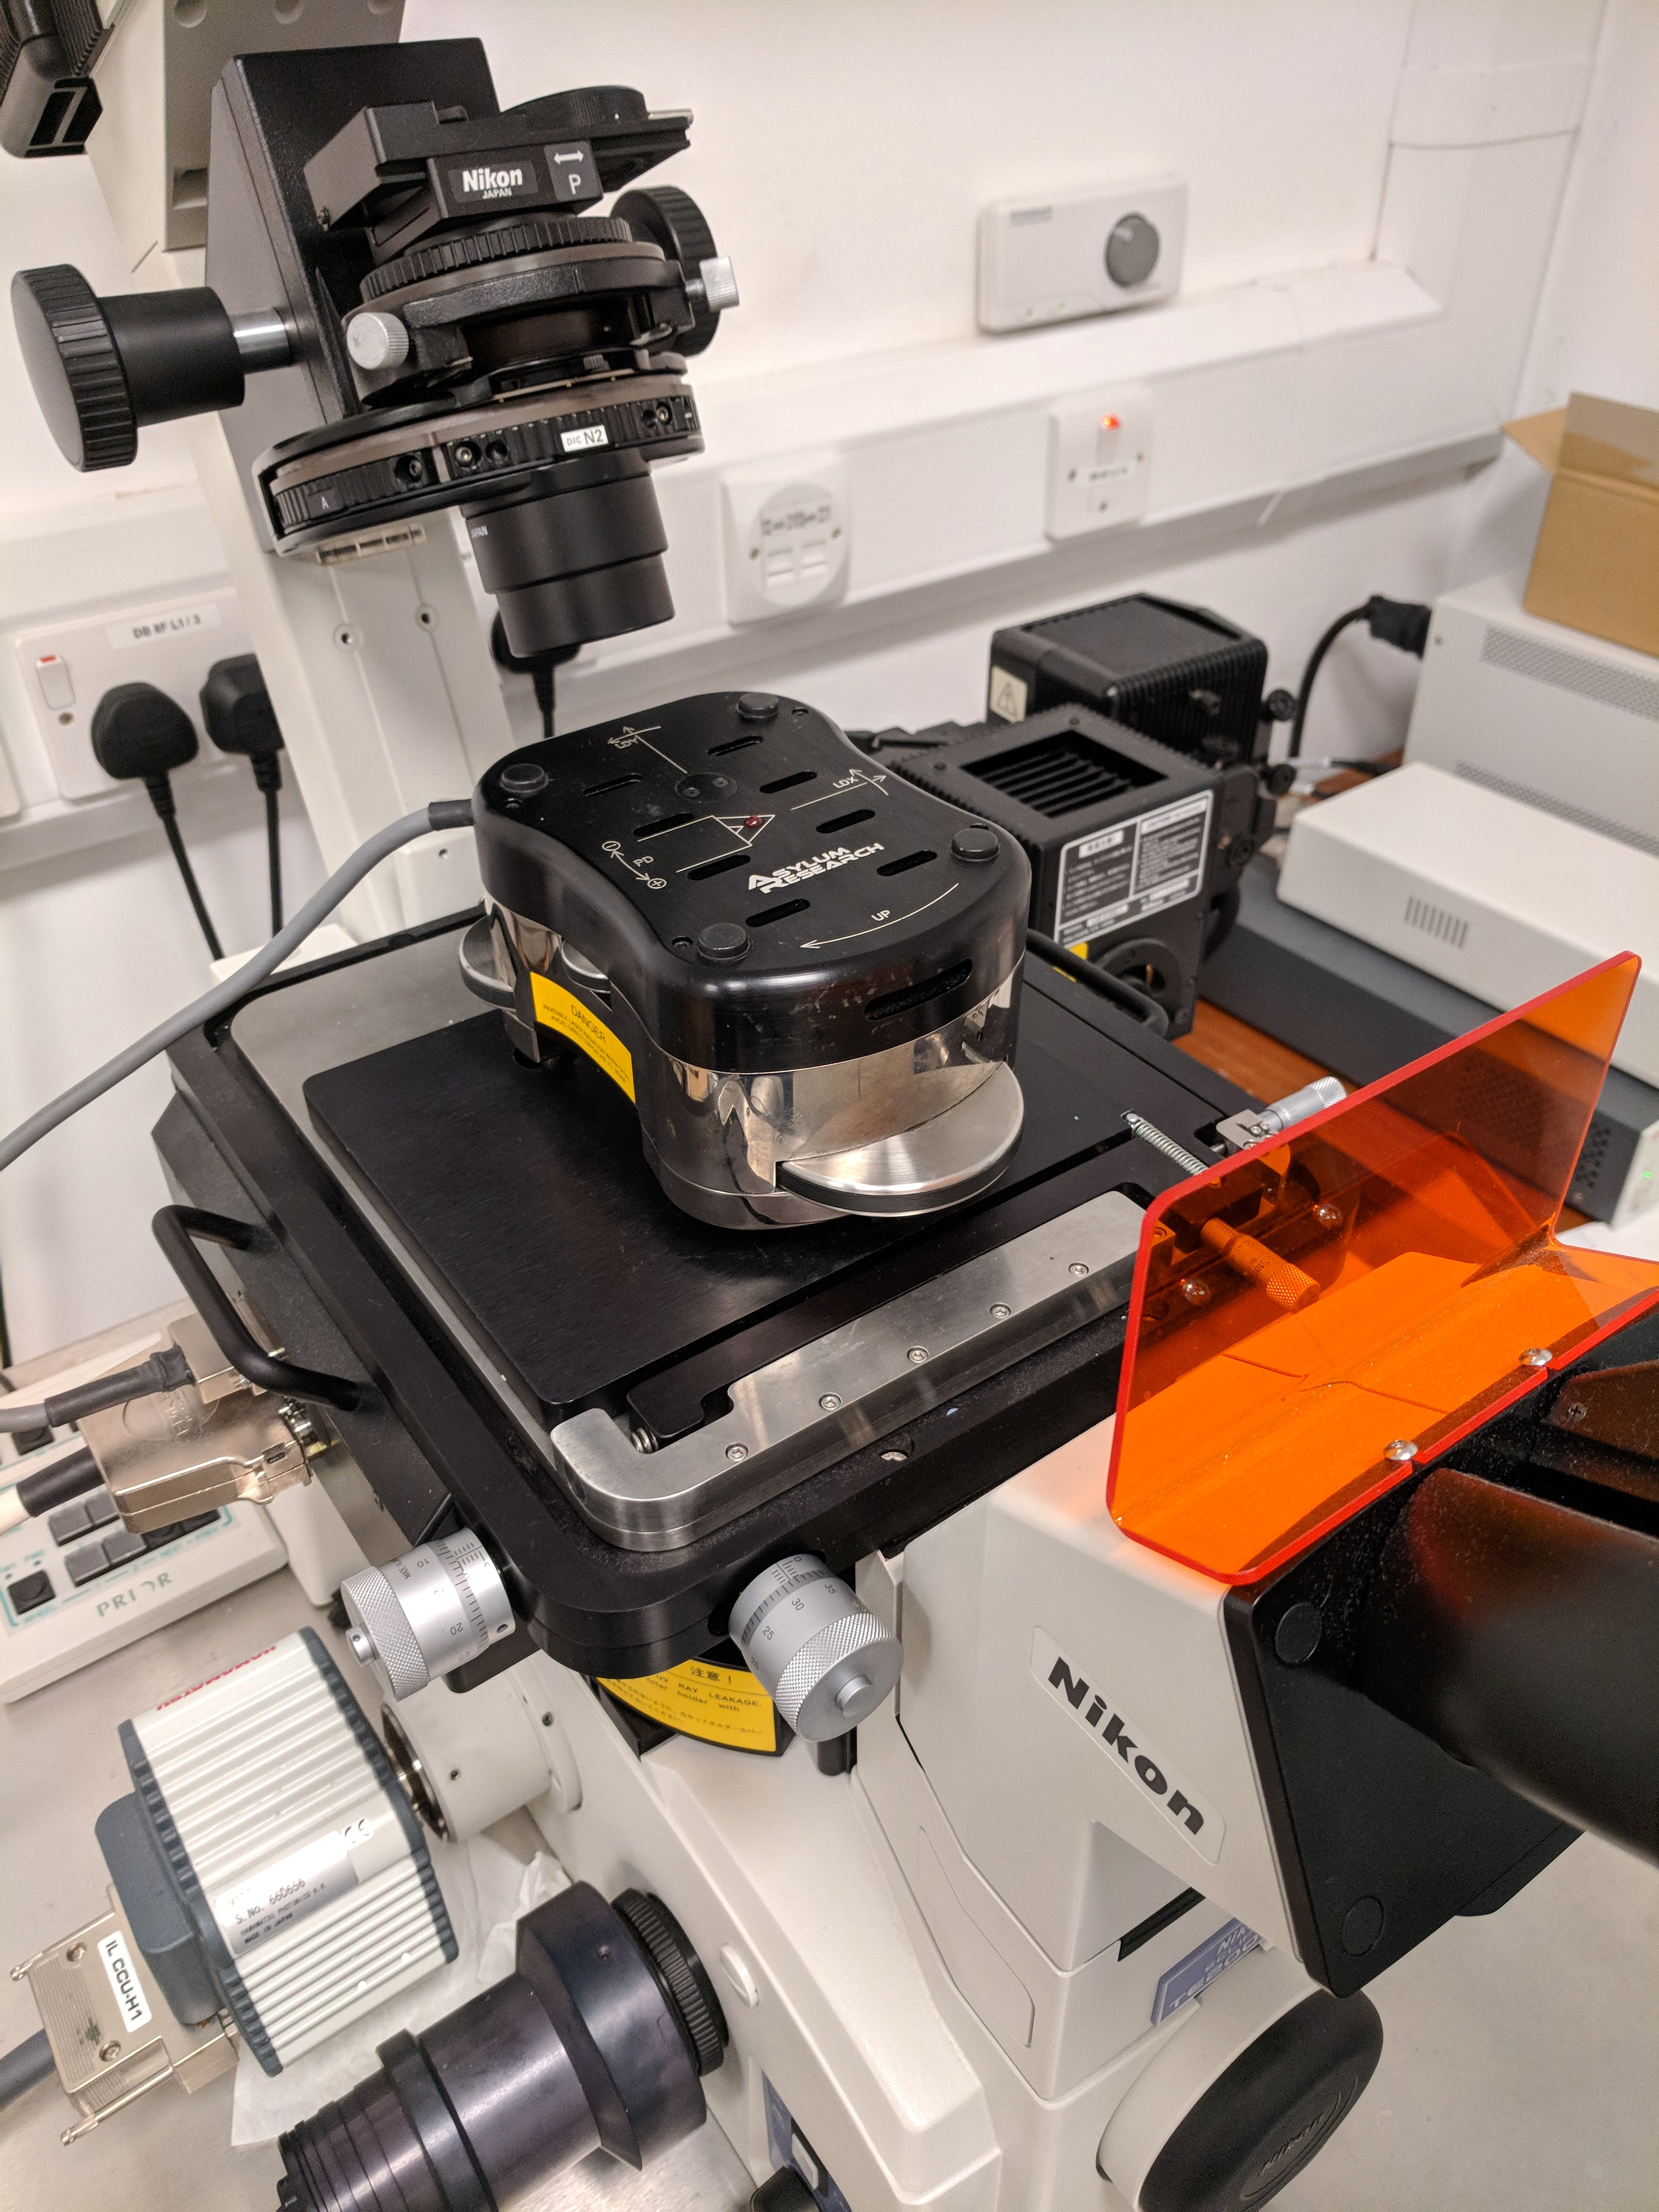
\includegraphics[width=80mm]{chapter2/forceAFM.jpg}
\end{center}
\caption{Operation setup for the MFP-1D AFM that was used for force measurements.}
\label{fig:forceAFM.jpg}                 % Reference label to the figure.
\end{figure}

For the force microscopy setup a MFP-1D from Asylum Research was used. The MFP-1D is an AFM mounted on top of an inverted light mircoscope, with the sample placed between the scanning head and the stage of the light microscope. In the AFM head the cantilever is mounted using tweezers in a holding apparatus. This head is immobile in the X,Y direction, horizontal movement is instead controlled by manlipulation of the stage. In the Z direction there are two possible movements - the 3 legs of the head can be moved vertically using the wheels for coarse movement, either to bring the tip in contact with the sample, or to level the head so the contact of the tip with the surface is uniform. The other control over the vertical height is via the piezoelectric transducer (piezo) mounted in the center of the head. This piezo has a travel range of roughly \SI{15}{\micro\metre}s. A laser is then emitted from inside the head and directed onto the cantlever, towards the sample. (See figure~\ref{fig:forceAFM.jpg})

For laser alignment on the AFM head an inverted microscope is used. First the cantilever is brought into focus under the microscope, then the position of the laser is aligned atop of the intended cantilever. Afterwards the laser is focused upon the center of the tip using the sum output given by the photosensitive diode. The diode converts photonic incident light into an output voltage, this allows the position of the laser focal point to be determined with respect to the diode boundaries.  Finally the deflection of the laser is set to 0; a central position between the positive and negative extremes. deviation of the laser's focal point from the center point of the photodiode allow movements of the cantilever to be detected. This  detect any bending (and thus attraction/repulsion) of the cantilever. 

In terms of the structure of the device, it differs slightly to the imaging AFM; the components are more tightly packed, mounted atop of the z-piezo directly, which then brings the apparatus down onto the sample, unlike the z-piezo raising the sample up to be imaged. In addition a Linear variable differential transformer (LVDT) sensor is mounted inside of the head to improve z-piezo accuracy \ref{fig:Head.jpg}

\begin{figure}[h!]     %Insert a figure as soon as possible
        \begin{center}
          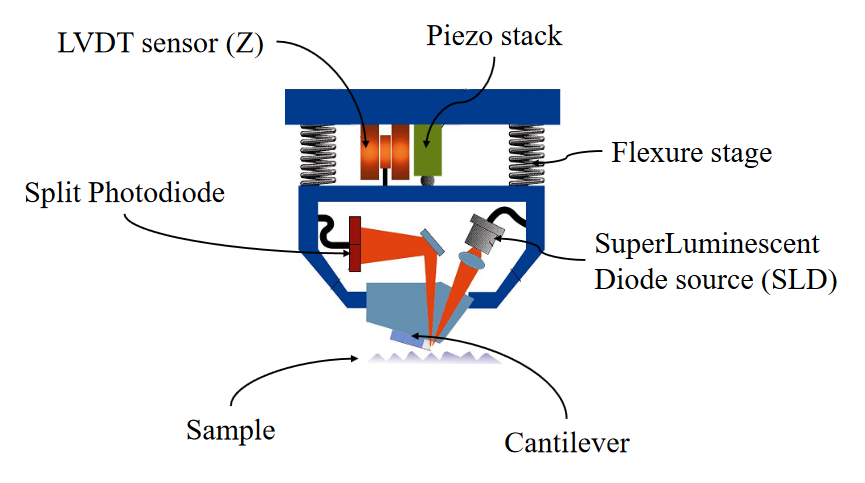
\includegraphics[width=80mm]{chapter2/Head.PNG}
\end{center}
\caption{Operational setup for the MFP-1D AFM that was used for force measurements. Adapted from \cite{AFMTalk}} %remake in joe style to reduce concerns
\label{fig:Head.jpg}                 % Reference label to the figure.
\end{figure}

%Add how vibrations in the building resolve into experimental noise and therefore dupe the system into thinking it's hit the surface.

Due to the feedback nature of the AFM, relying on previous data to define the voltage control from the next approach, the peak force (the intended maximum force applied on the cantilever per curve) was set to a relatively low number 8nN. This was done to limit the amount of tip damage during operation. In cases where the tip "loses" the surface, usually as a result of noise,  re-approach to be as gentle as possible. Additionally, the standard speed of tip movement was set to 1$\mu m/s$ (unless otherwise stated) to further reduce strain upon the tip.

\subsubsection{A note on noise}



\subsection{Experimental setup}

%Diagram of interaction

Initially the experimental setup was focused on investigating the interactions between two silica particles. Given the difficulty in aligning two micron sized particles for interaction, the first experimental setup involved using a silica particle glued to a cantilever (see fig \ref{Chapter3ExperiSetup}. These types of cantilevers are produced commercially, and were purchased to reduce experimental setup time. This cantilever was then brought into contact with a silica surface, with the results transformed using the Derjaguin approximation (See chapter 1). 

The first setup involved a 1.6$\mu$m diameter tip brought into contact with a silica surface glued to the  inside of a plastic petri dish. This setup allowed for a liquid solution to be placed on top of the surface, contained within the plastic petri dish. A 50:50 solution of deionised water and glycerol with a controlled concentration of LiCl was added. This solution was brought up to completely cover the tip, and ensure the head of the AFM was submerged.

The initial setup involved calibrating the cantilever tip on a separate calibration surface (see chapter 2), then removing this surface and replacing it with the experimental one. Initially approaching the surface was of little issue, but the greatest difficulty arose in finding contact with the surface under liquid. Given that the liquid in use was of a different optical density than air, the interface between the two was no longer visible under the microscope. As a result; the initial approach was slow, methodical and careful, as recklessness would break the tip. 

Problems with the setup were initially present, after a sweep of 4 different concentrations it was found that the resulting debye lengths for all the curves were above 6nm. These were directly contrary to the expectation that debye length should decrease to theoretically 0 at increasing salt concentrations.  The anomalous readings were considered to be the result of unidentified contaminants. Given the setup with the AFM was open by necessity as well as the difficulty in getting the sample under the tip in an expedient manner, there was little protection against airborne contaminants. Equally contaminants originating from the the plastic of the petri dish and glue were identified as a source of problems. The method of cleaning the surface was also called into question. %considering rewriting for flow

In order to address these issues, a few changes were implemented over a series of experiments. The surface used was exposed to an improved washing protocol. This washing protocol used deionised water to clean the surface over a greater period of time. Ethanol was considered, but due to the glue holding the surface down, there were concerns over the surface having a stable platform. Additionally the method of approach was revised slightly, with a large part of the distance between the surface and the tip performed in air, with the liquid solution injected using a glass pipette slowly. This injection relied on the surface tension of the water to slowly fill the dish, resulting in a slightly higher volume use. This was done to minimize any dramatic flow from damaging the tip, emulating a normal approach submerging mechanics. %Finally any glass wear use was limited to one use only instead of attempting to clean. - I mean that's kind of standard in anything, worth mentioning?

Contamination issues were still present after these revisions. In order to maximise contaminant removal, the plastic petri dish was replaced with a borosilica glass one. Instead of gluing a surface on top of the petri dish, the surface of the dish itself became the sampled area. While there had been previous considerations of the stability of the glue influencing the resulting force curve, the approach had been focused on solving the contaminant problem first. By using the surface of the dish itself, any concerns regarding glue induced artifacts could be laid to rest. This new dish permitted the use of ethanol in the cleaning procedure, as well as plasma treatment of the surface. The silica bead diameter on the cantilever was also increased to 6$\mu$m to increase the area to volume ratio.

The final protocol that was used is as follows: The glass petri dish and lid was cleaned with ethanol and water, followed by plasma treated. The lid was replaced immediately after, and remained on until use. The cantilever was mounted into the AFM head, and the laser aligned as closely as possible to the center on the photodiode. The petri dish was then put under the head, and it's blank surface was used to calibrate and calculate the spring constant of the cantilever. The cantilever was then retracted by a known amount, and then the liquid solution was the pipetted in. After the liquid had settled, the laser was recentered to adjust for the change in optical density. The tip was then brought into contact with the utmost care, relying on deflection readouts due to blind nature of the approach. Finally after contact, 100-200 curves were taken per site. If multiple sites were taken, the tip was retracted slowly, the petri dish moved slightly, and the approach phase was repeated. When transition between differing electrolyte concentrations, the tip is retracted, cleaned carefully with water, and plasma treated along with the petri dish. Otherwise the protocol was repeated. A tip was not plasma treated more than twice due to the degradation of the tip (see fig \ref{fig:ScorchedEarth}).

%Explain what plasma treatment is

\begin{figure}[h!]    
        \begin{center}
          \includegraphics[width=90mm]{chapter4/ScorchedEarth.png}
\end{center}
\caption{The view of a tip overtreated by plasma down the viewport of a microscope. Normally a tip is silver on the outside, but from over-treatment the surface is worn away.}
\label{fig:ScorchedEarth}                 
\end{figure}

Afterwards a final check was performed to see if the experimentally determined debye length matched our expectations. An approximation of the debye length ($\kappa$) was calculated using:

\begin{equation}
\kappa = \sqrt{\frac{\epsilon_r \epsilon_0 k_b T}{2 N_A e^2 I}}
\end{equation}

Where $\epsilon_r$ is the dielectric constant which was taken from \cite{WaterGlycerolEpR}. $\epsilon_0$ is the absolute dielectric permittivity. $k_b$ is the Boltzmann constant, $N_A$ is Avogadro's constant,  $e$ is the charge, $I$ is ionic strength and $T$ is temperature.

\begin{figure}[h!]    
        \begin{center}
          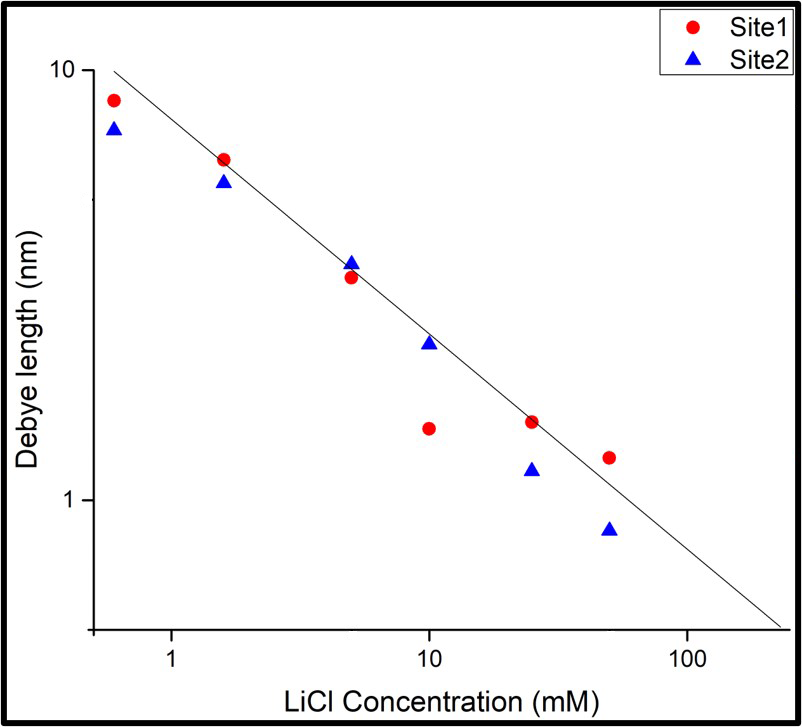
\includegraphics[width=110mm]{chapter4/DebyeLength.png}
\end{center}
\caption{A preliminary graph produced to investigate the expected debye length vs the recorded debye length at different salt concentrations. The black line indicates the approximated $\kappa$, whereas site one and two are two different recording areas on the glass surface.}
\label{fig:DebyeLength}                 
\end{figure}

This procedure produced sensible debye length measurements according to the preliminary data (see fig \ref{fig:DebyeLength}). As a result this procedure was used for subsequent experiments. These curves were used for analysis using the following script mechanics.

\newpage
%47.2 - glycerol
%


%Majority of the data collected to be around the inflection point -
%This was done to apply as little operational damage onto the cantilever. - Mention it again earlier, but less focus on the data output side.
%Mention the time factor - 0.5Hz 2s per curve. Earlier, with the experimental setup of the AFM
%Discuss in more detail about how the curve is taken though put it in chapter 2 !!
%fluctuations in the system cause the AFM to "lose" track of the surface and therefore increase the voltage input into the movement, over-correcting it's movement, shifting the captured area further up. After this the error correction it reduces the voltage until it stabilises.
%Hurricane Leslie ruining data due to location in the building.

\subsection{MFP-1D batch processing}

Using python\cite{python}, an automated script constructed to process the large volume of data generated by the MFP-1D AFM, given that each site generated around 100-200 approach and retract curves, and that multiple sites were used for each concentration, this produced a sizeable volume of data of around 6,000 curves which would be unmanageable without some form of automation.

%Overly fluffy
%A bit word salad-y too

%Make it less about the data
%appendix
For each measurement site, a minimum of 100 force curve readings per site was taken, with the raw data saved in a single file. The columns alternate with the raw deflection reading for one curve, followed by the corresponding z-piezo value. For the majority of readings the whole curve is measured throughout the reading, combining the approach and retract curves into one whole column. In the case where the cantilever is held at a certain location for a period of time, a new set of columns is appended, with another one starting after it begins movement again, thus fracturing the data whenever an acceleration/deceleration is applied to the cantilever.


From this each curve was broken down into two lists of raw unprocessed data given from the machine; the piezo height and the deflection. The piezo height is the recorded height of the cantilever on a scale of 0$\mu$m to 5$\mu$m. This range corresponds to the effective movement of the piezo head in the z direction, and is thus variable between datasets, as contact can be anywhere within this range. It is worth noting that the z height controlled by the legs of the AFM is independent, and is not measured by the machine. Contact is a result of the leg height being set by the operator manually, then the head coming into contact within it's 5$\mu$m range. The deflection is the deviation in nm from the calibrated equilibrium position, around the center of the photodiode. This deviation arises from when the cantilever is bent in a certain direction, causing the reflected laser off the top of the head to move along the photodiode's sensory range. These two lists were then saved in individual data files, with any derivative graphs following the same naming convention defined by the input file, with respect to unpacked bulk site curve set. 

%parameters:
%cfit_min
%cfit_max
%dfit_win
%dfit_off

%Rough script overview:
%Kc is calculated during AFM operation which is then added into the script by hand.

%Creation of output directory first, mfp.split_curves
%Then reads the csv if present, otherwise generates raw data files using
%mfp.comp_def_deriv
%mfp.proc_force_sep


%Afterwards plots the separation graphs with mfp.plot_force_sep_res
%Finally calculates contact forces with mfp.get_contact_forces

%mfp.split_curves
%Creates directories:
%force curves (master folder)
%raw force curves:
%- (force (N) / z piezo position (m)) %I.e. where the pizeo is in the range of it's movement (max 5um)
%Approach (see later)
%Retract (see later)

%(also removes velocity wave curves as there is only one taken at the start (and it's not always there for random reasons, but probably don't mention that)

%Decasualise 

These isolated files are then processed individually first, with several functions performed on the dataset. Using numpy an array is set up with the data present in the raw data file.

As it stands, this raw data requires at the bare minimum translation from a distance vs distance graph into a force vs distance graph.

Using numpy an array is set up with the data present in the raw data file.

Each of the curves per site is then split up into individual numpy arrays in preparation for the following functions. As it stands, this raw data requires at the bare minimum translation from a distance vs distance graph into a force vs distance graph. This corresponding graph is produced of force (nN)vs z-piezo position ($\mu$m). The raw deflection is converted into nanonewtons using the spring constant of the cantilever with the following equation.

\begin{equation}
F = Kc(\delta - \delta _{offset})1e^9
\end{equation}

Where F is force, Kc is the spring constant and $\delta$ is the deflection. %Unnecessary?

Equally the z-piezo position is converted into micrometers. This produces both a individual data file for ease of use on repeats, as several runs are expected to hone the parameters down to improve the quality of the analysis.  

\begin{figure}[h!]     %Insert a figure as soon as possible
        \begin{center}
          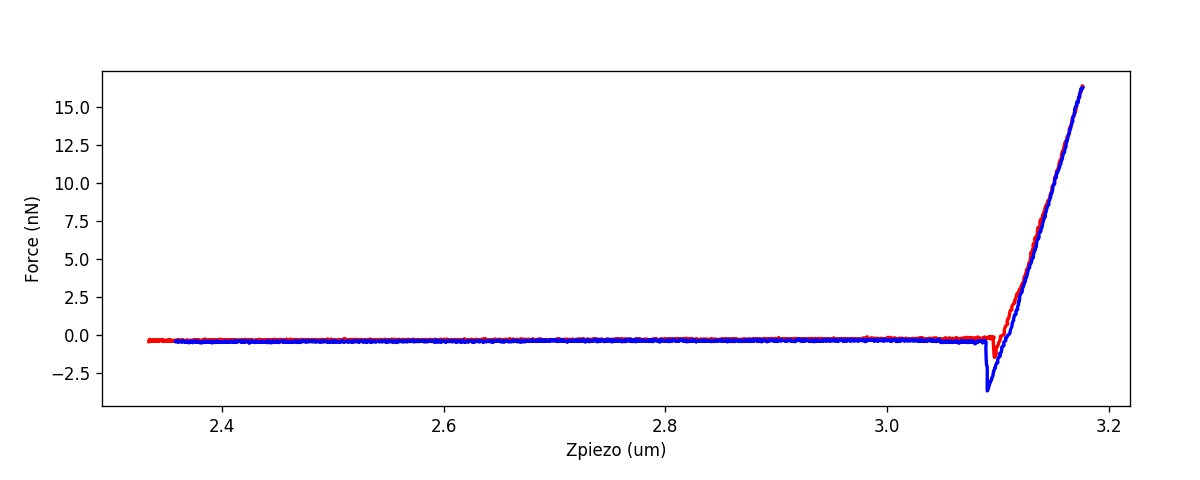
\includegraphics[width=110mm]{chapter4/EgRawGraph.jpg}
\end{center}
\caption{An example of a individual graph produced at this point. Minimal processing has been done with only the deflection converted into force (m to nN) and piezo z position m into $\mu$m}
\label{fig:EgRawGraph}                 % Reference label to the figure.
\end{figure}

The output is then checked over by eye. In some cases the resultant curve is not typical. This can arise when the cantilever doesn't move far enough down to find the surface, or when the cantilever starts in contact with the surface at the start of the movement. While these curves were rare, they did occur during standard use of the AFM, with erroneous curves usually corrected automatically by the AFM via error correction feedback. 

In order for the script to perform correctly on each of the curves, there needs to be a long enough stretch of data for the approach, and equally a long enough contact region. In the vast majority of cases this is true, there are a few cases where during normal operation an over correction occurs, resulting in the frame of reference to be shifted along the theoretical master curve. The operation parameters of the AFM aim to collect the most amount of data around the inflection point while reducing the amount of unneeded movement towards the surface, and equally reducing the amount of strain forced upon the cantilever during the contact region. At high strains the surface of the cantilever or petri dish can become damaged, or the cantilever can become damaged or break. As the conversion of deflection into force requires the spring constant to remain the same, and damage can cause this conversion to no longer remain true, any damage over the operation is considered by reviewing the curves over time. If there is a significant drift in the shape of the curve over the process of a site, then this is highlighted, or repeated. In the event of the cantilever breaking the AFM ceases to function, and therefore data collection stops.%usually followed by ample swearing

In some cases however, due to the feedback mechanism of the AFM defining the voltage input for the next step based off the previous step, and due to noise and uncontrollable factors (vibrations in the building for example) the frame of reference can shift up, resulting in an unusable curve, simple due to the lack of a data in a specific area. These fluctuations in the system cause the AFM to "lose" track of the surface and therefore increase the voltage input into the movement, over-correcting it's movement, shifting the captured area further up. After this the error correction it reduces the voltage until it stabilises. In addition, in the case of an uncontrollable error (primarily vibration based) the noise of a specific curve can throw off the normal processing of the script. It is in these instances that these curves are identified and removed.

%How I know a curve is not typical by eye. Example based approach?
%Show example bad graphs

%mfp.comp_def_deriv



%proc_force_sep() and comp_def_deriv() (?)
%guess contact point and work backwards, uses np.where
%cthresh = 'first pass' guess deflection threshold for contact. cthresh is set manually
%returns de-drifted zp, df.  data used to de-drift runs from dfit_win:2*dfit_win
%remove_farfield_drift()
Each curve is then processed individually. The first step taken is to address some of the background noise, this is done by taking a linear portion of the curve, where any movement done by the piezo is far enough away that any forces acting between the surface and the cantilever are zero. This removes any farfield drift, intending to remove any gradient found along the linear non-contact region. 

\begin{figure}[h!]     %Insert a figure as soon as possible
        \begin{center}
          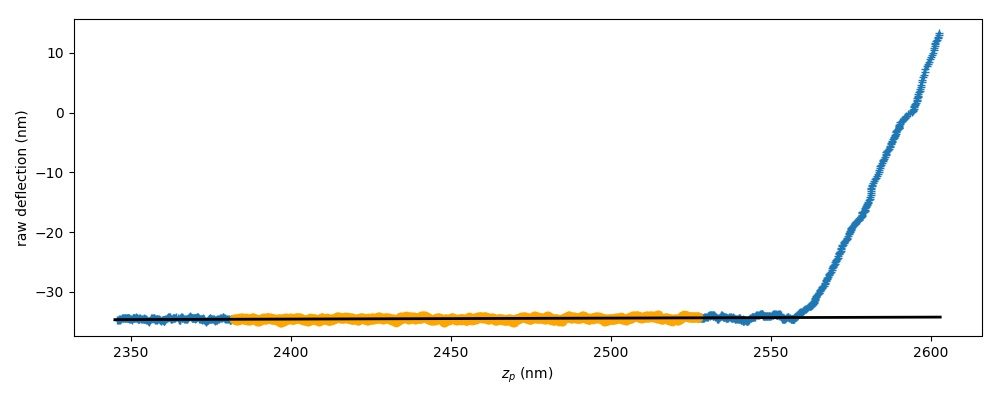
\includegraphics[width=110mm]{chapter4/farfielddrift.jpg}
\end{center}
\caption{An example of a individual graph produced for a single approach curve. The orange region of the graph is the area used in the farfield drift reduction and used to set the floor of the data to 0.}
\label{fig:farfielddrift}                 % Reference label to the figure.
\end{figure}


This area is defined by a region along this curve, set to use points away from the initial contact area of the curve. Initially the nm per datapoint is calculated by taking the range adjusted range of data divided by the total number of datapoints. From a combination of user input and estimating where the contact area is, and working backwards, the data window is set along this linear regime, with a respective graph produced to indicate what region is selected. This linear region is then floored, with the whole dataset translated up or down to the point where the region is at 0.
%remove_farfield_drift() end

Afterwards the data is then binned into a variable set. This value is determined by trail and error on a per case basis, but in most cases the bin size is 5. In earlier curves where the total number of data points taken was 2000 per curve, the bin size was smaller. Shortly afterwards the total number of points was increased to 8000. The objective of this set was to produce a smoother curve and reduce the effects of noise intrinsic to the system, this helps define where the contact point on the curve is.
%Why did I pick the bin sizes that I did
%(basically binning as much data as possible to smooth the curve without losing enough data points)
%Show multiple curves to show the effect of increasing bin size? Yeh bluergh

After binning, a first degree polynomial is fitted to the selected data. In the case where a suitable fit could not be found for the curve, this set is skipped, and the curve is left untranslated.

Our focus is then drawn to the area in which the tip has made contact with the surface, where any peizo movement is directly translated into cantilever deformation. In general, this range is defined by the operator by reviewing the graphical output from the previous steps, though an estimate is produced on the first run of the script (not sure if true, it just remembers the default if you don't input anything). This range aims to include as much as the graph as possible after the contact point, though it should be highlighted that the material in the cantilever is not uniform and therefore deformation is not a purely linear event in practice.

\begin{figure}[h!]    
        \begin{center}
          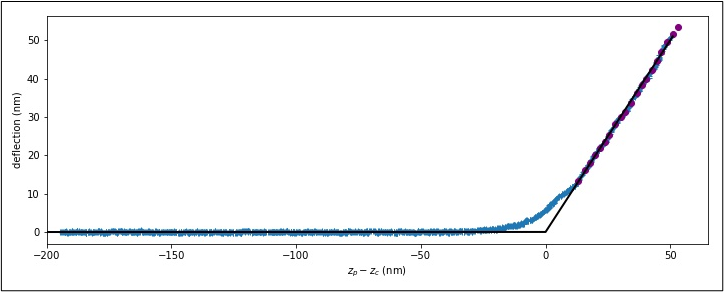
\includegraphics[width=110mm]{chapter4/contactRegion.png}
\end{center}
\caption{An example plot of an approach curve. The area used to define contact is highlighted by the purple dots overlaying the raw curve.} %word salad
\label{fig:contactRegion}                
\end{figure}

Using this defined region, we extrapolate back to the intercept and redefine this region as piezo position ($z_p$) - contact point ($z_c$). In the case that there is a jump to contact, the jump point is used instead of the interpolated $z_c$. Each curve is then normalised to 0 using this extrapolation. In the case where some individual curves have a high range of forces/deflection (usually as a result of overcompensating) this region of the graph is removed. This is because of the non-linear region intrinsic to the photodiode detector.

In order to ensure that the region defined by the operator is correct, a number of graphs are produced in order to aid the selection process. The deflection is derived in order to highlight the transition between the movement phase and the contact phase of the graph. This is done for individual curves as well as a averaged curve.

\begin{figure}[h!]    
        \begin{center}
          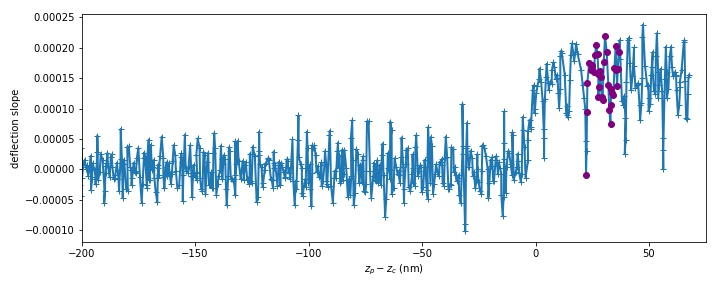
\includegraphics[width=110mm]{chapter4/EgInduDeriv.jpg}
\end{center}
\caption{An example plot of a derived approach curve. The area used to define contact is highlighted by the purple dots overlaying the raw curve. The black line indicates where the corrected baseline is, and where the extrapolated data intersects.}
\label{fig:EgInduDeriv}                
\end{figure}

\begin{figure}[h!]    
        \begin{center}
          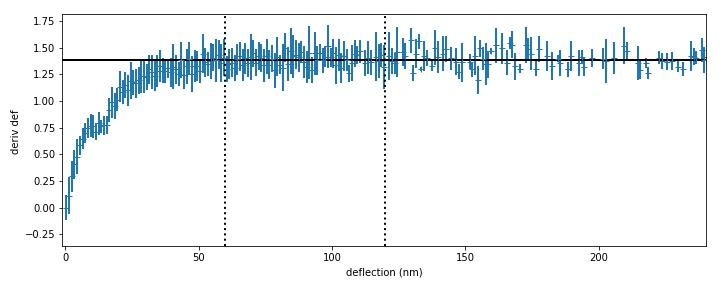
\includegraphics[width=110mm]{chapter4/EgAvgDeriv.jpg}
\end{center}
\caption{An example plot of the averaged derived approach curve. The area used to define contact is highlighted by dotted black lines. The horizontal black line indicates the extrapolation of the data. in this case the data is binned to reduce noise. The height of each blue bar indicates the standard deviation for each point.}
\label{fig:EgAvgDeriv}                
\end{figure}

\newpage

These curves are then all plotted on top of one another to check that all curves follow the same rough potential.

\begin{figure}[h!]     %Insert a figure as soon as possible
        \begin{center}
          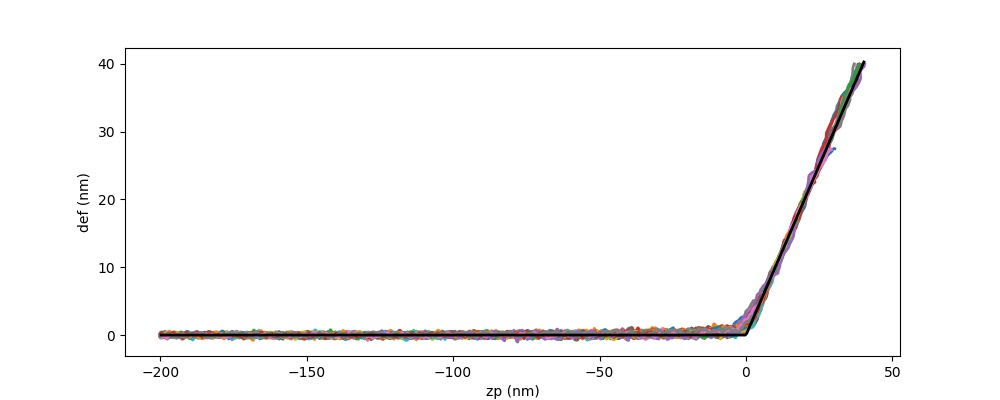
\includegraphics[width=110mm]{chapter4/proc_force_sep_mastercurve.jpg}
\end{center}
\caption{An example plot of all the curves processed up until this point. A reference black line is overlaid demonstrating what a curve would look like with no long range forces applied.}
\label{fig:proc_force_sep_mastercurve}                 % Reference label to the figure.
\end{figure}

%histogram of detection slope, not sure if it's worth mentioning, mostly a quick check to see nothing crazy happens

%#mfp.proc_force_sep END

%mfp.plot_force_sep_res 



This resolves in a final averaged and binned force curve (see fig \ref{fig:EgFinalCurve})

\begin{figure}[h!!!]     %Insert a figure as soon as possible
        \begin{center}
          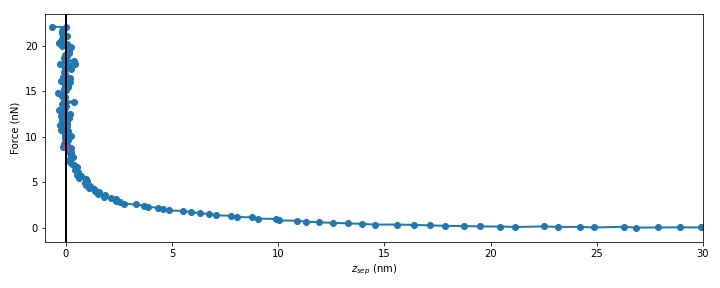
\includegraphics[width=110mm]{chapter4/EgFinalCurve.jpg}
\end{center}
\caption{An example plot of the final processed force curve. The y axis has been translated to show the distance from contact, with a black line highlighting the defined point of contact.}
\label{fig:EgFinalCurve}                 % Reference label to the figure.
\end{figure}

%mfp.get_contact_forces

Afterwards the focus of the script changes to calculating the force applied at contact. Positive forces indicate a repulsive force, negative forces indicate an attractive force. A Savitzky–Golay filter is applied to the data to reduce the noise intrinsic to the data. Then the curve is followed algorithmic until it passes over the threshold point - by default where separation is 0.

\newpage %goddamn tex and its graphs LATEX PLS

\begin{figure}[h!!!!!!!!!!!!!!!!!!!!!!!!!!!!]     %Insert a figure as soon as possible
        \begin{center}
          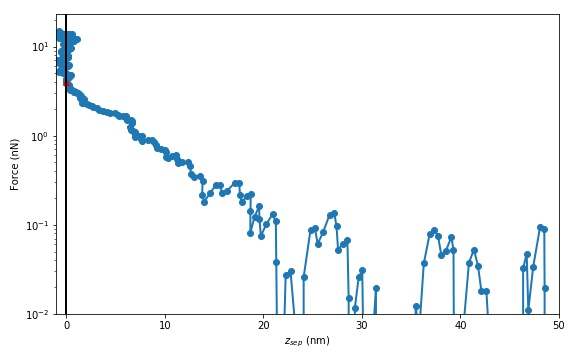
\includegraphics[width=110mm]{chapter4/LogLinEgForceContact.jpg}
\end{center}
\caption{An example plot of a log vs linear graph. The datapoint used to define the force at contact is highlighted in red with the black line defining contact.}
\label{fig:LogLinEgForceContact}                 % Reference label to the figure.
\end{figure}

This is done for each individual curve, eventually resulting in a histogram of of contact forces (fig \ref{fig:EgForceHisto}).

\begin{figure}[h!!!]     %Insert a figure as soon as possible
        \begin{center}
          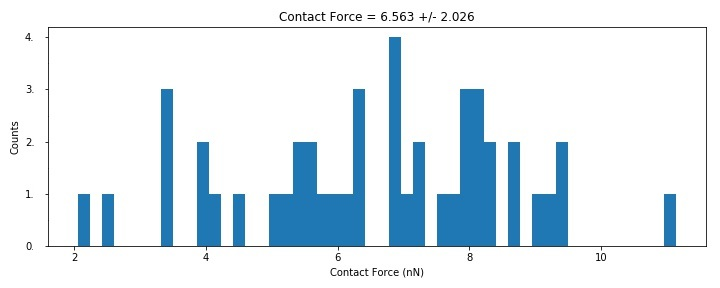
\includegraphics[width=110mm]{chapter4/EgForceHisto.jpg}
\end{center}
\caption{An example of a histogram produced. The mean force is given at the top with the standard deviation.}
\label{fig:EgForceHisto}                 % Reference label to the figure.
\end{figure}

In most cases the total number of individual graphs per final force datapoint is between 80-200 curves.

\newpage

\section{Nanowizard}

\begin{figure}[h!]     %Insert a figure as soon as possible
        \begin{center}
          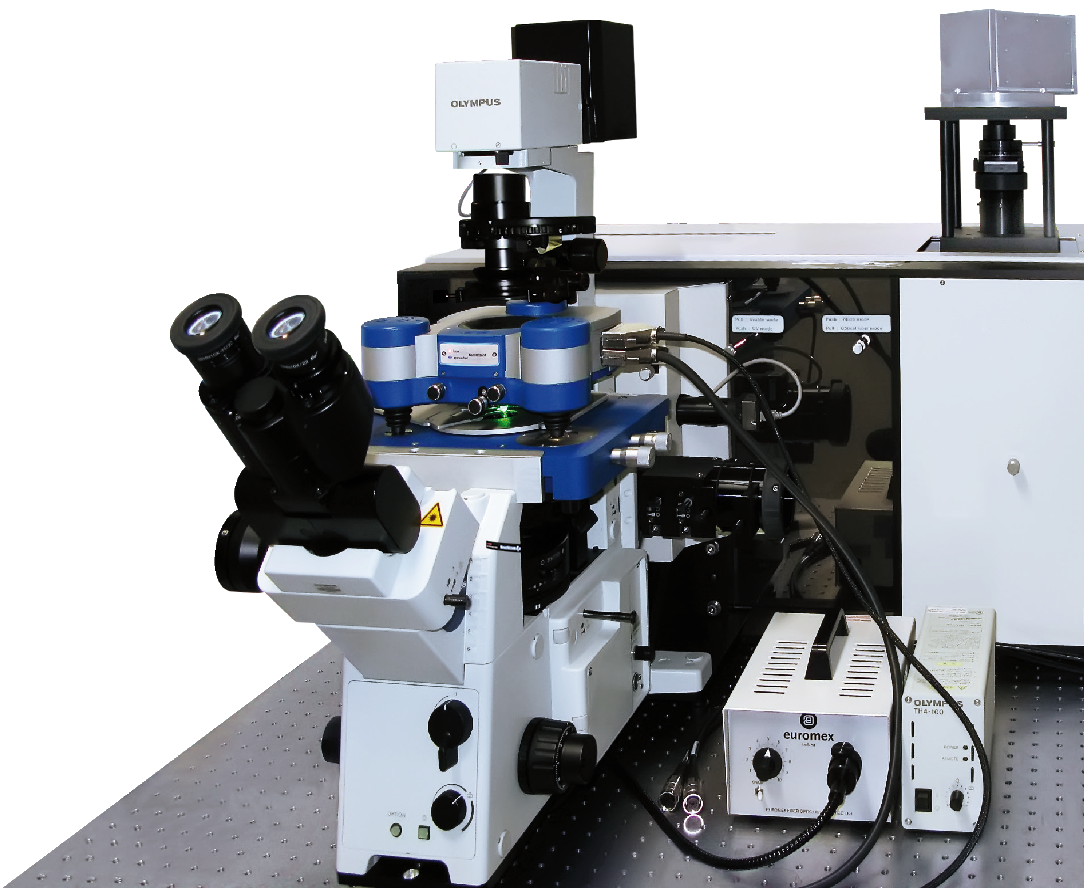
\includegraphics[width=80mm]{chapter4/Nanowizard.png}
\end{center}
\caption{Operation setup for the Nanowizard AFM that was used for force measurements \cite{NWizardPic}}
\label{fig:Nanowizard.png}                 % Reference label to the figure.
\end{figure}

Over the course of the investigation the availability of an alternative AFM became available. When compared to the MFP-1D, the setup is very similar, with one notable exception. This AFM allows for free x,y control coupled to the AFM head, instead of requiring the operator to disengage each time. Aside from the time saved between changing sites, this allows for techniques such as force mapping to be used (See chapter 2). The setup procedure remained the same as defined before during use with this AFM with any difference being software based, and thus an unnecessary detail for this report. 

Fortunately the previously established sample preparation, the cleaning procedure adapted with little difficulty and the expediency of operation was only improved with it's ease of use. The tip speed was set to the previously defined speed, 1$\mu m/s$ as well as the peak force at 8nN, unless otherwise stated.

\subsection{Analysis differences for JPK NanoWizard} %What is this an RPG tabletop for scientists?

The output from the Nanowizard was exported from the proprietary JPK file format and refitted to work with the script described above. While the differences in output structure is dramatic, this was handled by a short refactoring script to translate the data into a usable format. The only differences of note between the two is the JPK format providing a reduced significant figure and the deflection measured in N instead of m.

In the case of force mapping, there are considerably less curves per site. At this point, the previously established curves produced by the MFP-1D for each concentration are used for comparison. Each of the curves is then processed by the script, with a note taken of it's x,y $\mu$m offset. Afterwards the averaged contact force (for approach) or adhesive force (for retract) is plotted on a heat map. For each heat map a 10x10 grid was processed, with at minimum 3 curves per site taken, with a 1 $\mu$m distance between each site. It should be noted that the software processes an entire grid first, which is to say each site is repeated after all sites of the current grid are done.

%include any changes observed here. Only difference so far is that it's a faff and that the sig figs is lower on the JPK file format.


%%%Review later:




%%Insert graph showing selection window
%Possibly go into more detail
%Actually do
%Just not right now, your mind can't make sense of it



